% vim: set spell spelllang=en tw=100 :

\documentclass[sigconf]{acmart}

\usepackage{amsmath}
\usepackage{amssymb}
\usepackage{cleveref}
\usepackage{tikz}
\usepackage{nicefrac}

\usetikzlibrary{decorations, decorations.pathreplacing, calc, backgrounds}

\definecolor{uofgsandstone}{rgb}{0.321569, 0.278431, 0.231373}
\definecolor{uofglawn}{rgb}{0.517647, 0.741176, 0}
\definecolor{uofgcobalt}{rgb}{0, 0.615686, 0.92549}
\definecolor{uofgpumpkin}{rgb}{1.0, 0.72549, 0.282353}
\definecolor{uofgthistle}{rgb}{0.584314, 0.070588, 0.447059}

% cref style
\crefname{figure}{Figure}{Figures}
\Crefname{figure}{Figure}{Figures}

\newcommand{\citepos}[1]{\citet{#1}'s}

% pretty colours
\definecolor{uofgsandstone}{rgb}{0.321569, 0.278431, 0.231373}
\definecolor{magmapurple}{rgb}{0.505882, 0.145098, 0.505882}
\definecolor{magmaorange}{rgb}{0.984314, 0.529412, 0.380392}

% http://tex.stackexchange.com/questions/22100/the-bar-and-overline-commands
\newcommand{\shortoverline}[1]{\mkern 1.5mu\overline{\mkern-1.5mu#1\mkern-1.5mu}\mkern 1.5mu}

\newcommand*\samethanks[1][\value{footnote}]{\footnotemark[#1]}

% Copyright
%\setcopyright{none}
%\setcopyright{acmcopyright}
%\setcopyright{acmlicensed}
\setcopyright{rightsretained}
%\setcopyright{usgov}
%\setcopyright{usgovmixed}
%\setcopyright{cagov}
%\setcopyright{cagovmixed}


% DOI
\acmDOI{10.475/123_4}

% ISBN
\acmISBN{123-4567-24-567/08/06}

%Conference
\acmConference[IA$^3$ 2017]{Seventh Workshop on Irregular Applications: Architectures and Algorithms}{November 2017}{Denver, Colorado USA}
\acmYear{2017}
\copyrightyear{2017}

\acmPrice{666.00}

\begin{document}
\title[Observations from Parallelising Three Subgraph Algorithms]{Observations from Parallelising Three Maximum Common (Connected) Subgraph Algorithms}
\titlenote{This work was supported by the Engineering and Physical Sciences
    Research Council [grant numbers EP/K503058/1, EP/M508056, and EP/P026842/1] and the ANR project
SoLStiCe (ANR-13-BS02-0002-01)}

\author{Ruth Hoffmann}
\affiliation{%
    \institution{University of St Andrews}
    \city{St Andrews, Scotland}
}

\author{Ciaran McCreesh}
\affiliation{%
    \institution{University of Glasgow}
    \city{Glasgow, Scotland}
}
\email{ciaran.mccreesh@glasgow.ac.uk}

\author{Samba Ndojh Ndiaye}
\affiliation{
    \institution{Universit\'e Lyon 1, LIRIS, UMR5205}
    \city{F-69621, France}
}

\author{Patrick Prosser}
\affiliation{%
    \institution{University of Glasgow}
    \city{Glasgow, Scotland}
}

\author{Craig Reilly}
\affiliation{%
    \institution{University of Glasgow}
    \city{Glasgow, Scotland}
}

\author{Christine Solnon}
\affiliation{
    \institution{INSA-Lyon, LIRIS, UMR5205}
    \city{F-69621, France}
}

\author{James Trimble}
\affiliation{%
    \institution{University of Glasgow}
    \city{Glasgow, Scotland}
}

% The default list of authors is too long for headers}
\renewcommand{\shortauthors}{R. Hoffmann, C. McCreesh et al.}

\begin{abstract}
    We discuss our experiences adapting three recent algorithms for maximum common (connected)
    subgraph problems to exploit multi-core parallelism. These algorithms are heavily irregular and
    very sensitive to search order changes, and so do not easily lend themselves to parallel search.
    Nonetheless, our results show that each algorithm can be parallelised successfully, with the
    multi-core algorithms we create being clearly better than the sequential ones. We then look in
    more detail at the results, and discuss how we should be
    measuring speedups for these kinds of algorithm. Because of the difficulty in measuring an
    average speedup when so-called anomalous (superlinear and sublinear) speedups are common, we
    propose a new measure called \emph{aggregate speedup}.
\end{abstract}

\begin{CCSXML}
<ccs2012>
<concept>
<concept_id>10003752.10003809.10003716.10011136</concept_id>
<concept_desc>Theory of computation~Discrete optimization</concept_desc>
<concept_significance>500</concept_significance>
</concept>
<concept>
<concept_id>10003752.10003809.10010170</concept_id>
<concept_desc>Theory of computation~Parallel algorithms</concept_desc>
<concept_significance>500</concept_significance>
</concept>
<concept>
<concept_id>10003752.10003809.10011254.10011256</concept_id>
<concept_desc>Theory of computation~Branch-and-bound</concept_desc>
<concept_significance>500</concept_significance>
</concept>
<concept>
<concept_id>10003752.10003790.10003795</concept_id>
<concept_desc>Theory of computation~Constraint and logic programming</concept_desc>
<concept_significance>300</concept_significance>
</concept>
</ccs2012>
\end{CCSXML}

\ccsdesc[500]{Theory of computation~Discrete optimization}
\ccsdesc[500]{Theory of computation~Parallel algorithms}
\ccsdesc[500]{Theory of computation~Branch-and-bound}
\ccsdesc[300]{Theory of computation~Constraint and logic programming}

\keywords{Maximum common subgraph, Parallel branch and bound}

\maketitle

\section{Introduction}

\begin{figure}[b]
    \centering
    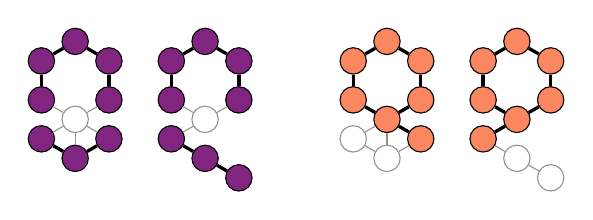
\begin{tikzpicture}[scale=0.33]%{{{
        \begin{scope}
            \node[draw, circle, fill=magmapurple, inner sep=0.5pt, font=\normalsize] (M1) at (90:1.5) {\phantom{0}};
            \node[draw, circle, fill=magmapurple, inner sep=0.5pt, font=\normalsize] (M2) at (150:1.5) {\phantom{0}};
            \node[draw, circle, fill=magmapurple, inner sep=0.5pt, font=\normalsize] (M3) at (30:1.5) {\phantom{0}};
            \node[draw, circle, fill=magmapurple, inner sep=0.5pt, font=\normalsize] (M4) at (210:1.5) {\phantom{0}};
            \node[draw, circle, fill=magmapurple, inner sep=0.5pt, font=\normalsize] (M5) at (330:1.5) {\phantom{0}};
            \node[draw, circle, draw=uofgsandstone!60, fill=white, inner sep=0.5pt, font=\normalsize] (M6) at (270:1.5) {\phantom{0}};
            \node[draw, circle, fill=magmapurple, inner sep=0.5pt, font=\normalsize] (M7) at ($(210:1.5) + (M6)$) {\phantom{0}};
            \node[draw, circle, fill=magmapurple, inner sep=0.5pt, font=\normalsize] (M8) at ($(330:1.5) + (M6)$) {\phantom{0}};
            \node[draw, circle, fill=magmapurple, inner sep=0.5pt, font=\normalsize] (M9) at ($(270:1.5) + (M6)$) {\phantom{0}};

            \draw [very thick] (M1) -- (M2);
            \draw [very thick] (M2) -- (M4);
            \draw [very thick] (M3) -- (M5);
            \draw [color=uofgsandstone!60] (M4) -- (M6);
            \draw [color=uofgsandstone!60] (M5) -- (M6);
            \draw [very thick] (M3) -- (M1);
            \draw [color=uofgsandstone!60] (M6) -- (M7);
            \draw [color=uofgsandstone!60] (M6) -- (M8);
            \draw [color=uofgsandstone!60] (M6) -- (M9);
            \draw [very thick] (M7) -- (M9);
            \draw [very thick] (M8) -- (M9);
        \end{scope}

        \begin{scope}[xshift=5cm]
            \node[draw, circle, fill=magmapurple, inner sep=0.5pt, font=\normalsize] (M1) at (90:1.5) {\phantom{0}};
            \node[draw, circle, fill=magmapurple, inner sep=0.5pt, font=\normalsize] (M2) at (150:1.5) {\phantom{0}};
            \node[draw, circle, fill=magmapurple, inner sep=0.5pt, font=\normalsize] (M3) at (30:1.5) {\phantom{0}};
            \node[draw, circle, fill=magmapurple, inner sep=0.5pt, font=\normalsize] (M4) at (210:1.5) {\phantom{0}};
            \node[draw, circle, fill=magmapurple, inner sep=0.5pt, font=\normalsize] (M5) at (330:1.5) {\phantom{0}};
            \node[draw, circle, draw=uofgsandstone!60, fill=white, inner sep=0.5pt, font=\normalsize] (M6) at (270:1.5) {\phantom{0}};
            \node[draw, circle, fill=magmapurple, inner sep=0.5pt, font=\normalsize] (M7) at ($(210:1.5) + (M6)$) {\phantom{0}};
            \node[draw, circle, fill=magmapurple, inner sep=0.5pt, font=\normalsize] (M8) at ($(270:1.5) + (M6)$) {\phantom{0}};
            \node[draw, circle, fill=magmapurple, inner sep=0.5pt, font=\normalsize] (M9) at ($(330:1.5) + (M8)$) {\phantom{0}};

            \draw [very thick] (M1) -- (M2);
            \draw [very thick] (M2) -- (M4);
            \draw [very thick] (M3) -- (M5);
            \draw [color=uofgsandstone!60] (M4) -- (M6);
            \draw [color=uofgsandstone!60] (M5) -- (M6);
            \draw [very thick] (M3) -- (M1);
            \draw [color=uofgsandstone!60] (M6) -- (M7);
            \draw [very thick] (M7) -- (M8);
            \draw [very thick] (M8) -- (M9);
        \end{scope}

        \begin{scope}[xshift=12cm]
            \node[draw, circle, fill=magmaorange, inner sep=0.5pt, font=\normalsize] (M1) at (90:1.5) {\phantom{0}};
            \node[draw, circle, fill=magmaorange, inner sep=0.5pt, font=\normalsize] (M2) at (150:1.5) {\phantom{0}};
            \node[draw, circle, fill=magmaorange, inner sep=0.5pt, font=\normalsize] (M3) at (30:1.5) {\phantom{0}};
            \node[draw, circle, fill=magmaorange, inner sep=0.5pt, font=\normalsize] (M4) at (210:1.5) {\phantom{0}};
            \node[draw, circle, fill=magmaorange, inner sep=0.5pt, font=\normalsize] (M5) at (330:1.5) {\phantom{0}};
            \node[draw, circle, fill=magmaorange, inner sep=0.5pt, font=\normalsize] (M6) at (270:1.5) {\phantom{0}};
            \node[draw, circle, draw=uofgsandstone!60, fill=white, inner sep=0.5pt, font=\normalsize] (M7) at ($(210:1.5) + (M6)$) {\phantom{0}};
            \node[draw, circle, fill=magmaorange, inner sep=0.5pt, font=\normalsize] (M8) at ($(330:1.5) + (M6)$) {\phantom{0}};
            \node[draw, circle, draw=uofgsandstone!60, fill=white, inner sep=0.5pt, font=\normalsize] (M9) at ($(270:1.5) + (M6)$) {\phantom{0}};

            \draw [very thick] (M1) -- (M2);
            \draw [very thick] (M2) -- (M4);
            \draw [very thick] (M3) -- (M5);
            \draw [very thick] (M4) -- (M6);
            \draw [very thick] (M5) -- (M6);
            \draw [very thick] (M3) -- (M1);
            \draw [color=uofgsandstone!60] (M6) -- (M7);
            \draw [very thick] (M6) -- (M8);
            \draw [color=uofgsandstone!60] (M6) -- (M9);
            \draw [color=uofgsandstone!60] (M7) -- (M9);
            \draw [color=uofgsandstone!60] (M8) -- (M9);
        \end{scope}

        \begin{scope}[xshift=17cm]
            \node[draw, circle, fill=magmaorange, inner sep=0.5pt, font=\normalsize] (M1) at (90:1.5) {\phantom{0}};
            \node[draw, circle, fill=magmaorange, inner sep=0.5pt, font=\normalsize] (M2) at (150:1.5) {\phantom{0}};
            \node[draw, circle, fill=magmaorange, inner sep=0.5pt, font=\normalsize] (M3) at (30:1.5) {\phantom{0}};
            \node[draw, circle, fill=magmaorange, inner sep=0.5pt, font=\normalsize] (M4) at (210:1.5) {\phantom{0}};
            \node[draw, circle, fill=magmaorange, inner sep=0.5pt, font=\normalsize] (M5) at (330:1.5) {\phantom{0}};
            \node[draw, circle, fill=magmaorange, inner sep=0.5pt, font=\normalsize] (M6) at (270:1.5) {\phantom{0}};
            \node[draw, circle, fill=magmaorange, inner sep=0.5pt, font=\normalsize] (M7) at ($(210:1.5) + (M6)$) {\phantom{0}};
            \node[draw, circle, draw=uofgsandstone!60, fill=white, inner sep=0.5pt, font=\normalsize] (M8) at ($(270:1.5) + (M6)$) {\phantom{0}};
            \node[draw, circle, draw=uofgsandstone!60, fill=white, inner sep=0.5pt, font=\normalsize] (M9) at ($(330:1.5) + (M8)$) {\phantom{0}};

            \draw [very thick] (M1) -- (M2);
            \draw [very thick] (M2) -- (M4);
            \draw [very thick] (M3) -- (M5);
            \draw [very thick] (M4) -- (M6);
            \draw [very thick] (M5) -- (M6);
            \draw [very thick] (M3) -- (M1);
            \draw [very thick] (M6) -- (M7);
            \draw [draw=uofgsandstone!60] (M7) -- (M8);
            \draw [draw=uofgsandstone!60] (M8) -- (M9);
        \end{scope}
\end{tikzpicture}
\caption{A maximum common subgraph of the first two graphs has eight vertices, shaded. A maximum
common \emph{connected} subgraph, shown on the right, has only seven vertices.}
\label{figure:mcsexample}
\end{figure}

A \emph{subgraph isomorphism} is an injective mapping from a \emph{pattern} graph to a \emph{target}
graph which maps adjacent vertices to adjacent vertices---that is, it \emph{preserves adjacency}. It
is \emph{induced} if additionally it maps non-adjacent vertices to non-adjacent vertices, preserving
non-adjacency. When working with labelled graphs, a subgraph isomorphism must preserve labels, and
on directed graphs, it must preserve orientation. A \emph{common induced subgraph} of two graphs $G$
and $H$ is a pair of induced subgraph isomorphisms from a pattern graph $P$, one to $G$ and one to
$H$. A \emph{maximum common induced subgraph} is one with as many vertices as possible.

Finding a maximum common subgraph is the key step in measuring the similarity or difference between
two graphs \citep{DBLP:journals/prl/Bunke97,DBLP:journals/prl/FernandezV01,o:Kriege15}: to determine
the difference between two graphs, we find what they have in common, and then take everything left
over. Because of this, maximum common subgraph problems frequently arise in biology and chemistry
\citep{DBLP:journals/jcamd/RaymondW02a,o:EhrlichR11,DBLP:journals/dam/GayFMSS14} where graphs
represent molecules, but also in applications including computer vision
\citep{DBLP:journals/jair/CookH94,DBLP:conf/gbrpr/CombierDS13}, computer-aided manufacturing
\citep{o:LuoWSN17}, crisis management \citep{o:DelavalladeFLL16}, deanonymising datasets
\citep{o:SharadD13}, the analysis of source code \citep{DBLP:journals/tkde/DjokoCH97} and binary
programs \citep{DBLP:conf/icics/GaoRS08}, in
malware detection \citep{DBLP:journals/compsec/ParkRS13}, social network analysis
\citep{DBLP:journals/tkde/FangYZZ15}, graph database query explanations
\citep{DBLP:journals/jcss/VasilyevaTBL16}, and in character recognition problems
\citep{DBLP:journals/pr/LuRS91}.  A common variant of the problem requires a largest
\emph{connected} subgraph
\citep{DBLP:journals/tcs/Koch01,DBLP:journals/jcamd/RaymondW02a,DBLP:conf/mco/VismaraV08,o:EhrlichR11,o:LuoWSN17}.
As illustrated in \cref{figure:mcsexample}, a maximum common connected subgraph cannot be determined
from the maximum common subgraph.

Although both variants are NP-hard, some progress has been made towards solving the problem in
practice.  This paper looks at three recent branch and bound algorithms for maximum common
(connected) induced subgraph problems, each of which is the state of the art for certain classes of
instance. We discuss our experiences in adding parallel tree-search to these three algorithms. In
each case, our results show that the parallel version of the algorithm is clearly better than the
sequential version, although a closer look at the results shows many nuances.

\section{Sequential Algorithms}

There are three competitive approaches for the maximum common subgraph problem, each being the
strongest on certain classes of instance. The first involves a reduction to the maximum clique
problem, whilst the other two approaches have a constraint programming feel to them.

\subsection{Reduction to Maximum Clique}

A clique in a graph is a subgraph where every vertex is adjacent to every other. There is a
well-known reduction from the maximum common subgraph problem to the problem of finding a maximum
clique in an \emph{association graph}
\citep{o:Levi73,DBLP:journals/jcamd/RaymondW02a,DBLP:conf/cp/McCreeshNPS16}, which, when combined with
a modern maximum clique solver \citep{DBLP:journals/ol/SegundoMRH13}, is the current best approach for
solving the problem on labelled graphs \citep{DBLP:conf/cp/McCreeshNPS16}. A modified clique-like
algorithm can also be used to solve the maximum common connected subgraph problem, by ensuring
connectedness during search \citep{DBLP:conf/cp/McCreeshNPS16}; again, this is the best known way of
solving the problem on labelled graphs.

A major downside of the maximum clique approach is that the association graph encoding is extremely
memory-intensive, limiting its practical use to pairs of graphs with no more than a few hundred
vertices.

\subsection{Constraint Programming}

The maximum common subgraph problem may be reformulated as a constraint optimisation problem, as
follows.  Observe that an equivalent definition of a common subgraph of graphs $G$ and $H$ is an
injective \emph{partial} mapping from $G$ to $H$ which preserves both adjacency and non-adjacency.
Hence we pick whichever input graph has fewer vertices, and call it the \emph{pattern}; the other
graph is called the \emph{target}. The model then follows from this new definition: for each vertex
in the pattern, we create a variable, whose domain ranges over each vertex in the target graph, plus
an additional value $\bot$ representing an unmapped vertex. We then have three sets of constraints.
The first set says that for each pair of adjacent vertices in the pattern (that is, for each edge in
the pattern), if neither of these vertices are mapped to $\bot$ then these vertices must be mapped
to an adjacent pair of target vertices. The second set is similar, but looks at non-adjacent pairs
(or non-edges).  Finally, the third set ensures injectivity, by enforcing that the variables must be
all different except when using $\bot$. This final set of constraints may either be implemented
using binary constraints between all pairs of variables, or a special global ``all different except
$\bot$'' propagator \citep{DBLP:conf/cp/PetitRB01}. The objective is simply to find an assignment of
values to variables, maximising the number of variables not set to $\bot$. The state of the art for
this technique is a dedicated implementation of a forward-checking branch and bound search over this
model \citep{DBLP:conf/cp/NdiayeS11,DBLP:conf/cp/McCreeshNPS16}.

Two approaches exist for ensuring connectedness: either a conventional global constraint and
propagator can be used \citep{DBLP:conf/cp/McCreeshNPS16}, or a special branching rule can be used
to enforce connectedness during search \citep{DBLP:conf/mco/VismaraV08}. The two techniques are
broadly comparable performance-wise \citep{DBLP:conf/cp/McCreeshNPS16}, but the branching rule is
much simpler to implement.

\subsection{Domain Splitting}

\citet{o:McCreeshPT17} observe that due to the special structure of the maximum common subgraph
problem, the following property holds throughout the search process using the constraint programming
model: any two variables either have domains with no values in common (with the possible exception
of $\bot$), or have identical domains. The McSplit algorithm exploits this property. It explores
essentially the same search tree as the basic forward-checking constraint programming model, but
using different supporting algorithms and data structures.  Rather than storing a domain for each
vertex in the pattern graph, equivalence classes of vertices in both graphs are stored in a special
data structure which is modified in-place and restored upon backtracking. This enables fast
propagation of the constraints and smaller memory requirements. In addition, this data structure
enables stronger branching heuristics to be calculated cheaply. The McSplit algorithm effectively
dominates conventional constraint programming approaches, being consistently over an order of
magnitude faster.

\subsection{$k$-less Subgraph Isomorphism}

A different take on the constraint programming model is presented by
\citet{DBLP:conf/aaai/HoffmannMR17}. They approach the maximum common subgraph via the
subgraph isomorphism problem, asking the question ``if a pattern graph cannot be found in the
target, how much of the pattern graph can be found?''. The $k{\downarrow}$ algorithm tries to solve
the subgraph isomorphism problem first for $k=0$ (asking whether the whole pattern graph can be found in the
target). Should that be not satisfiable, it tries to solve the problem for $k=1$ (one vertex cannot
be matched), and should that also not be satisfiable, it iteratively increases $k$ until the result
is satisfiable. The advantage of this approach is that strong invariants using paths and the degrees
of vertices may be used to prune large portions of the search space.

This algorithm is aimed primarily at large instances, where the two graphs are of different orders,
and where it is expected that the solution will involve most of the smaller graph (that is, $k$ is
expected to be low). The implementation we work with only handles unlabelled instances, and does
not support the connected variant.

\section{Benchmark Instances}

Most of the benchmark instances we will use come from a standard database for maximum common
subgraph problems \citep{DBLP:journals/prl/SantoFSV03,DBLP:journals/jgaa/ConteFV07}. This benchmark
set can be used in a number of ways, for different variants of the problem. We use it to create five
families of instance, as follows:

\begin{description}
    \item[Unlabelled] instances, by selecting the first ten members of each parameter class where the
        graphs have up to 50 vertices each---this gives us a total of 4,110 instances.

    \item[Vertex labelled] instances, by selecting the first ten members of each parameter class
        (and so graphs have up to 100 vertices each), applying the 33\% labelling scheme for
        vertices only, and treating edges as undirected. This gives 8,140 instances.

    \item[Both labelled, directed] instances, by selecting the first ten members of each parameter
        class, and applying the 33\% labelling scheme to both vertices and edges. Again, this gives
        8,140 instances.

    \item[Unlabelled, connected] instances, using the same instances as the \emph{unlabelled} case.

    \item[Both labelled, connected] instances, starting in the same way as the \emph{both labelled,
        directed} case. These are then converted to undirected graphs by treating edges as
        undirected, picking the label of the lower-numbered edge.
\end{description}

\noindent
Following \citet{DBLP:conf/aaai/HoffmannMR17}, we also work with the 5,725 \textbf{Large} instances
originally used for studying portfolios of subgraph isomorphism algorithms
\citep{DBLP:conf/lion/KotthoffMS16}. These graphs are unlabelled and undirected, and can include up
to 6,671 vertices. We do not use the clique encoding on these instances due to its
memory requirements.

\section{Parallel Search}

The clique and $k{\downarrow}$ algorithms already make use of fine granularity bit-parallelism. To
introduce more coarse-grained thread parallelism, we will parallelise the search process: viewing
backtracking search as forming a tree, we can explore different portions of the tree using different
threads. We use a shared incumbent, so better solutions found by one thread can be used others
immediately. This technique has a long history \citep{o:BaderHC05}. Of particular
interest to us are so-called \emph{anomalies}
\citep{DBLP:journals/cacm/LaiS84,DBLP:journals/tc/LiW86,DBLP:conf/irregular/BruinKT95}:
because we are not performing a fixed amount of work, we should have no expectation of a linear
speedup, and instead we could see a sublinear speedup (much less than $n$ from $n$ processors) or a
superlinear speedup (much more than $n$ from $n$ processors). An absolute slowdown (speedup much
less than 1) is also possible under some models.

\subsection{Parallel Maximum Clique}

Thread-parallel versions of state-of-the-art maximum clique algorithms have already been produced
\citep{DBLP:journals/algorithms/McCreeshP13,DBLP:journals/jcisd/DepolliKRTJ13,DBLP:conf/icde/XiangGA13}.
\citet{DBLP:journals/topc/McCreeshP15} compare several of these approaches, and make an important
observation: although work balance is a problem due to the irregularity of the search tree, often
the interaction between search order and parallel work decomposition is the dominating factor in
determining speedups. They explain why anomalies are in fact common in practice: many clique problem
instances benefit immensely from having found a strong incumbent, but have solutions which are
either unique or rare, and are hard to find. They propose a work splitting mechanism which offsets
anomalies, guaranteeing reproducibility (two runs with the same instance on the same hardware will
give similar runtimes), scalability (increasing the number of cores cannot make things worse), and
no absolute slowdowns.  Additionally, this mechanism explicitly offsets the commitment to early
branching choices, where search ordering heuristics are most likely to be inaccurate
\citep{DBLP:conf/ijcai/HarveyG95,DBLP:conf/cp/ChuSS09}.

We will use this mechanism for our experiments.  The clique-based maximum common subgraph algorithm
effectively differs only in the preprocessing stage, and the clique-inspired connected algorithm
described by \citet{DBLP:conf/cp/McCreeshNPS16} is sufficiently similar that may be parallelised in
exactly the same way. Based upon preliminary experiments, we use a splitting depth limit of five
rather than the original three, since maximum common subgraph instances appear to be even more
irregular than normal clique problem instances.

\subsection{Parallel Constraint-Based Search}

A similar approach may be used for the $k{\downarrow}$ algorithm. Although it is not quite a
conventional branch and bound algorithm, each individual $k$ pass is a tree search, and may be
parallelised. For each pass, we use the same work splitting mechanism as in the clique algorithm,
starting by splitting only at the top level of search to explicitly introduce diversity, and then
iteratively increasing the splitting depth as additional work is needed (up to a limit of five
levels deep).

Because the $k{\downarrow}$ algorithm uses a conventional constraint programming domain store, there
is no need to use recomputation; the state is naturally copied at each branching point.

In principle the McSplit algorithm may be parallelised in exactly the same way. However, this
algorithm makes heavy use of an in-place, backtrackable data structure, which is not copied for
recursive calls. In order to introduce the \emph{potential} for parallelism, we must make
copies of the state data structure. Implemented na{\"\i}vely, this can give an order of magnitude
slowdown to the sequential algorithm, which can be hard to recover using parallelism. To lessen the
effects, rather than copying state for each recursive call, we copy once before the main branching
loop, and then copy that copy in each ``helper'' thread, replaying the branching loop without making
duplicate recursive calls.  (We are not convinced that a better approach is not possible\ldots)

\section{Empirical Evaluation}

We perform our experiments on systems with dual Intel Xeon E5-2640 v2 processors and 64GBytes RAM,
running Ubuntu 14.04, with GCC 5.3.0 as the compiler. Each machine has a total of sixteen cores, and
hyper-threading is enabled, so we run experiments with 32 threads except where otherwise noted, but
we do not expect speedups of 32 even in the best case.

?? Hundred second timeout.

\subsection{Parallel Search is Better Overall}

\begin{figure*}[p]
    \includegraphics*{gen-graph-cumulative-plain.pdf}
    \hfill
    \includegraphics*{gen-graph-cumulative-33v.pdf}
    \hfill
    \includegraphics*{gen-graph-cumulative-33ved.pdf}

    \vspace*{1em}

    \includegraphics*{gen-graph-cumulative-plain-connected.pdf}
    \hfill
    \includegraphics*{gen-graph-cumulative-33ve-connected.pdf}
    \hfill
    \includegraphics*{gen-graph-cumulative-sip.pdf}

    \caption{The cumulative number of instances solved over time, for different families and
    algorithms. The 32 threaded parallel versions (shown using dotted lines) are always better in
aggregate than the sequential versions (shown using solid lines).}\label{figure:cumulative}
\end{figure*}

\begin{figure*}[p]
    \includegraphics*{gen-graph-scatter-plain-clique-vs-clique-par-t32.pdf}
    \hfill
    \includegraphics*{gen-graph-scatter-33v-clique-vs-clique-par-t32.pdf}
    \hfill
    \includegraphics*{gen-graph-scatter-33ved-clique-vs-clique-par-t32.pdf}
    \hfill
    \includegraphics*{gen-graph-scatter-plain-connected-clique-vs-clique-par-t32.pdf}
    \hfill
    \includegraphics*{gen-graph-scatter-33ve-connected-clique-vs-clique-par-t32.pdf}

    \vspace*{1em}

    \includegraphics*{gen-graph-histogram-plain-clique-vs-clique-par-t32.pdf}
    \hfill
    \includegraphics*{gen-graph-histogram-33v-clique-vs-clique-par-t32.pdf}
    \hfill
    \includegraphics*{gen-graph-histogram-33ved-clique-vs-clique-par-t32.pdf}
    \hfill
    \includegraphics*{gen-graph-histogram-plain-connected-clique-vs-clique-par-t32.pdf}
    \hfill
    \includegraphics*{gen-graph-histogram-33ve-connected-clique-vs-clique-par-t32.pdf}

    \caption{On the top row, per-instance speedups, using the clique algorithm. The $x$-axis is
    sequential performance and the $y$-axis is 32 threaded performance, so points below the diagonal
    line represent a speedup. Darker points represent instances where the solution is relatively
    large compared to the order of the input graphs. Below, histograms plotting the distribution of
    speedups for instances whose sequential runtime was at least 500 milliseconds, and below the
    timeout.}\label{figure:cliquespeedups}
\end{figure*}

In \cref{figure:cumulative} we plot empirical cumulative distribution functions showing the number
of instances solved over time, for both sequential (solid lines) and parallel (dotted lines)
versions of each algorithm.  Cumulative plots are commonly used in constraint programming and
boolean satisfiability for comparing aggregate behaviour of solvers in the presence of timeouts.
(Sometimes the axes are reversed, in which case they are called \emph{cactus} plots.)  To read these
plots, make a choice of timeout along the $x$-axis, which uses a log scale. The $y$ value at that
point shows the number of instances whose runtime (individually) is at most $x$, for a particular
algorithm. In other words, at any given $x$ value, the highest line shows which algorithm is able to
solve the largest number of instances using a per-instance timeout of that $x$ value, bearing in
mind that the actual sets of instances solved by each algorithm may be completely different.

Each plot gives the same conclusion: if we are working with a timeout of at least $10^2$
milliseconds, then for any problem family and any sequential algorithm, if given the option of
switching to the corresponding parallel algorithm, then we should do so.

However, although they are good at showing general trends, cumulative plots can hide interesting
details. We therefore now take a closer look at each of the three algorithms.

\subsection{Clique Results In Depth}

\begin{figure}[p]
    \includegraphics{gen-graph-as-clique.pdf}

    \caption{Aggregate speedups from 32 threads on 16 hyper-threaded cores, shown as a function of
    sequential runtime, for each family supported by the clique algorithm.}\label{figure:cliqueas}
\end{figure}
\begin{figure}[p]
    \includegraphics*{gen-graph-scatter-33ved-clique-vs-clique-par-t2.pdf}
    \hfill
    \includegraphics*{gen-graph-scatter-33ved-clique-par-t2-vs-clique-par-t4.pdf}

    \vspace*{1em}

    \includegraphics*{gen-graph-scatter-33ved-clique-par-t4-vs-clique-par-t8.pdf}
    \hfill
    \includegraphics*{gen-graph-scatter-33ved-clique-par-t8-vs-clique-par-t16.pdf}

    \vspace*{1em}

    \includegraphics*{gen-graph-scatter-33ved-clique-par-t16-vs-clique-par-t32.pdf}
    \hfill
    \includegraphics*{gen-graph-scatter-33ved-clique-par-t32r-vs-clique-par-t32.pdf}

    \caption{Per-instance speedups from the clique algorithm on vertex- and edge-labelled, directed
    instances, when going from sequential to two threads in the first plot, then increasing the
    number of threads in subsequent plots. The final plot shows 32 threads versus a repeated run
    also with 32 threads.}\label{figure:cliquescale}
\end{figure}

In the top row of \cref{figure:cliquespeedups}, we see scatter plots comparing the sequential and
parallel runtimes of the clique algorithm on an instance by instance basis, using a log-log plot.
Instances which timed out using one algorithm but not the other are shown as points along the outer
axes. Points below the $x{-}y$ diagonal line represent speedups. The colour of the points indicates
the relative size of the solution---darker points represent instances where the solution uses most
of the vertices of the input graphs. (We use these conventions for scatter plots throughout this
paper.)

Broadly speaking, the results are similar on each of the five families. For runtimes below 100
milliseconds, overheads and the preprocessing step dominate, and we are usually only able to achieve
a small speedup. At higher runtimes, most speedups appear to be between ten and twenty, except on
the final family, where they are mostly between five and ten. For a few instances, the speedups are
lower (but they are still clearly speedups), whilst in the first four families, we also see evidence
of super-linear speedups being relatively common.

However, attempting to determine a speedup by staring at a scatter plot is not particularly
quantitative. We could attempt to find a best fit line through these points, pretending that the
superlinear speedups are outliners. We could perhaps get away with this if outliers were rare
enough, but in practice we are not expecting linear speedups, and for the other two algorithms, we
will see that superlinear speedups are even more common. Alternatively, we could rig our experiments
to remove anomalies, by priming search with a known-optimal
solution---\citet{DBLP:journals/topc/McCreeshP15} criticise this practice in more detail.

A more principled approach is given in the bottom row of \cref{figure:cliquespeedups}. For instances
where the sequential run both succeeded and took at least 500 milliseconds, we plot the distribution
of speedups obtained. These histograms confirm our informal observations. However, these plots are
not particularly satisfactory: in order to calculate a speedup, we can only consider instances where
the sequential algorithm succeeded. These plots therefore underestimate superlinear speedups.

To avoid this weakness, we propose a new way of characterising speedups. Refer back to the
cumulative plots in \cref{figure:cumulative}. The usual way of comparing two algorithms on these
plots is to measuring the vertical difference between lines, which says how many more instances the
parallel algorithm can solve than the sequential algorithm can with a particular choice of timeout.
However, measuring the \emph{horizontal} distance between lines also conveys information. Suppose
the sequential algorithm can solve $y$ instances with a selected timeout of $s$. By moving to the
left on a cumulative plot, we can find the timeout $p$ required for the parallel algorithm to solve
the same number of instances, bearing in mind that \emph{the two sets of instances could in
principle have completely different members}. We therefore define the \emph{aggregate speedup} to be
$\nicefrac{s}{p}$; this can be expressed as a function of time (i.e.\ $s$) or of the number of
instances solved ($y$).

We plot aggregate speedups as a function of time in \cref{figure:cliqueas}. For a sequential timeout
of one hundred seconds, we get speedups of twenty to twenty eight in the unlabelled, vertex
labelled, and both labelled, directed cases. In the unlabelled connected case, our aggregate speedup
is thirty seven, which (when taking hyper-threading into account) is strongly super-linear.  With
some detailed knowledge of the underlying sequential algorithm, this should perhaps not surprise us:
for instances with a large solution, once we have found that solution, a proof of optimality is
relatively easy. However, finding that solution can be unusually hard, particularly since the
branching strategy for the connected constraint necessarily interferes with the tailored search
order used by modern clique algorithms.  In contrast, for the both labelled connected case, our
aggregate speedup is only six. A closer inspection of the results shows that the search tree is
unusually narrow and deep for these instances, making work balance harder and contention higher.

What about scalability and reproducibility? The first plot in \cref{figure:cliquescale} show the
effects of going from sequential to threaded with two cores, and the next four plots show the
effects of doubling the number of threads each time. These plots show that most of the superlinear
effects occur with fairly small numbers of threads, with nearly all of the benefits of increased
diversity in search being obtained once eight threads are used. As expected, in no case does
increasing the number of threads make things substantially worse, although going from sixteen to
thirty two threads does show some small slowdowns---this is due to hyper-threading.

The final plot in \cref{figure:cliquescale} shows that runtimes are reproducible: running the same
instance on the same hardware twice takes almost exactly the same amount of time. (We could not
reproduce the three outliers in a third run---we suspect other system programs may have woken up
and caused slight interference during the second run.)

These results are hopefully comforting: they show that anomalies can be controlled, and that
switching to a parallel algorithm is not only better, but also safe from a scientific
reproducibility perspective.

\subsection{$k{\downarrow}$ Results In Depth}

\begin{figure}[tb]
    \includegraphics*{gen-graph-scatter-plain-kdown-vs-kdown-par-t32.pdf}
    \hfill
    \includegraphics*{gen-graph-scatter-sip-kdown-vs-kdown-par-t32.pdf}

    \vspace*{1em}

    \includegraphics{gen-graph-as-kdown.pdf}

    \vspace*{1em}

    \includegraphics*{gen-graph-scatter-plain-kdown-par-t4-vs-kdown-par-t16.pdf}
    \hfill
    \includegraphics*{gen-graph-scatter-plain-kdown-par-t32r-vs-kdown-par-t32.pdf}

    \caption{On the top row, per-instance speedups, using the $k{\downarrow}$ algorithm. The
    $x$-axis is sequential performance and the $y$-axis is 32 threaded performance. Below,
    aggregate speedups for both families. Finally, scalability and reproducibility.}\label{figure:kdownscatters}
\end{figure}

In \cref{figure:kdownscatters} we show per-instance and aggregate speedups for the $k{\downarrow}$
algorithm. On unlabelled instances, we see a range of speedups between slightly less than one and
ten, with an aggregate speedup of four. These results are not as good as with the clique algorithm.
A closer look at the results suggests that memory bandwidth is to blame: although we have somewhat
more than sixteen times as much processing power available to us, our available memory bandwidth at
best doubles from introducing parallelism. Unlike the clique algorithm, which has very small,
cache-friendly data structures which are modified in-place, the state for the $k{\downarrow}$
algorithm is large and much of the runtime is spent copying data structures.

For the large instances, our aggregate speedup is higher, at over ten. This has two causes: for
larger graphs, the computational effort per recursive call increases by more than the amount the
memory copying does, reducing the memory bandwidth problem slightly, and additionally a much larger
number of super-linear speedups occurred with this family of instances. We could perhaps anticipate
this latter effect: in many of these instances the maximum common subgraph covers all or nearly all
of the smaller of the two graphs, and so once it is found, the proof of optimality is trivial.
However, finding a witness can be difficult. We should also expect value ordering heuristics in
these algorithms to be weak at the top of search (they are based upon degree, and many graphs do not
have a large degree spread), and so the benefits of high-up diversity can be extremely large
\citep{DBLP:conf/ijcai/HarveyG95,DBLP:conf/cp/ChuSS09,DBLP:journals/topc/McCreeshP15}. Indeed,
similar results were seen with a parallel version of the subgraph isomorphism algorithm upon which
$k{\downarrow}$ is based \citep{DBLP:conf/cp/McCreeshP15}.

The final row of \cref{figure:kdownscatters} shows that as with the clique algorithm, this
parallelism is reproducible, and that runtimes do not get worse when the number of threads is
increased. (Although not shown, we also tried to parallelise $k{\downarrow}$ using randomised
work-stealing from Intel Cilk Plus---similar to the clique algorithm
\citep{DBLP:journals/topc/McCreeshP15}, doing so gives generally reasonable results on average, but
now repeat runtimes can differ by more than an order of magnitude.)

\subsection{McSplit Results In Depth}

\begin{figure}[tb]
    \includegraphics*{gen-graph-scatter-plain-mcsplit-vs-mcsplit-par-t32.pdf}
    \hfill
    \includegraphics*{gen-graph-scatter-33v-mcsplit-vs-mcsplit-par-t32.pdf}

    \vspace*{1em}

    \includegraphics*{gen-graph-scatter-33ved-mcsplit-vs-mcsplit-par-t32.pdf}
    \hfill
    \includegraphics*{gen-graph-scatter-plain-connected-mcsplit-vs-mcsplit-par-t32.pdf}

    \vspace*{1em}

    \includegraphics*{gen-graph-scatter-33ve-connected-mcsplit-vs-mcsplit-par-t32.pdf}
    \hfill
    \includegraphics*{gen-graph-scatter-sip-mcsplit-vs-mcsplit-par-t32.pdf}

    \caption{Per-instance speedups, using the splitting algorithm. The $x$-axis is sequential
    performance and the $y$-axis is 32 threaded performance.}\label{figure:mcsplitscatter}
\end{figure}

Finally, we look at our attempts to parallelise the McSplit algorithm. Recall that doing so required
heavy modifications to the algorithm, introducing significant amounts of speculative copying of a
data structure that is usually backtrackable and modified in-place. \Cref{figure:mcsplitscatter}
shows ?? what?

?? Aggregate speedups in \cref{figure:mcsplitas}. Also show scalability and reproducibility.

\begin{figure}[tb]
    \includegraphics{gen-graph-as-mcsplit.pdf}

    \vspace*{1em}

    \includegraphics*{gen-graph-scatter-plain-mcsplit-par-t4-vs-mcsplit-par-t16.pdf}
    \hfill
    \includegraphics*{gen-graph-scatter-plain-mcsplit-par-t32r-vs-mcsplit-par-t32.pdf}

    \caption{On the top row row, aggregate speedups for the McSplit algorithm. Below, scalability
    and reproducibility.}\label{figure:mcsplitas}
\end{figure}

% \subsection{Cilk}
%
% \begin{figure}[tb]
%     \includegraphics*{gen-graph-scatter-33ved-clique-par-t32r-vs-clique-par-t32.pdf}
%     \hfill
%     \includegraphics*{gen-graph-scatter-33ved-clique-cilk-t32r-vs-clique-cilk-t32.pdf}
%
%     \vspace*{1em}
%
%     \includegraphics*{gen-graph-scatter-sip-kdown-par-t32r-vs-kdown-par-t32.pdf}
%     \hfill
%     \includegraphics*{gen-graph-scatter-sip-kdown-cilk-t32r-vs-kdown-cilk-t32.pdf}
%
%     \caption{Reproducibility using Cilk.}
% \end{figure}

\section{Conclusion}

?? There is more to be done.

?? Note the very high number of recursive calls per second. Fitting everything in cache. Not
compatible with framework abstractions. Recomputation versus state copying.

?? Aggregate speedups. Use of multiple measures.

?? Same algorithm, different instance families, very sensitive

\bibliographystyle{ACM-Reference-Format}
\bibliography{combined}

\end{document}
